

\QCMautoevaluation{Pour chaque question, plusieurs réponses sont proposées. Déterminer celles qui sont correctes.}

\begin{QCM}
  \begin{GroupeQCM}
    \begin{exercice}
    
\begin{center}      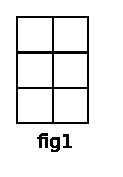
\includegraphics[width=1.4cm]{fig1} 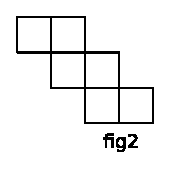
\includegraphics[width=2.2cm]{fig2}  \end{center}
      \begin{ChoixQCM}{4}
      \item Ces deux figures ont la même aire
      \item Ces deux figures ont le même périmètre
      \item Le périmètre de la figure 2 est plus grand que celui de la figure 1
      \item L'aire de la figure  2 est plus grande que l'aire de la figure 1
      \end{ChoixQCM}
\begin{corrige}
     \reponseQCM{ac} 
   \end{corrige}
    \end{exercice}


    \begin{exercice}
      Mon aire est de 4 cm\up{2} et mon périmètre est de 8 cm. Qui puis‑je être ?
      \begin{ChoixQCM}{4}
      \item Je suis un carré de côté 2 cm
      \item Je suis un rectangle de longueur 3 cm et de largeur 1 cm
      \item Je suis un rectangle de longueur 4 cm et de largeur 1 cm
      \item Je suis un carré de côté 4 cm
      \end{ChoixQCM}
\begin{corrige}
     \reponseQCM{a}
   \end{corrige}
    \end{exercice}
    
    
    \begin{exercice}
      Quelle(s) phrase(s) te semble(nt) raisonnable(s) ?
      \begin{ChoixQCM}{4}
      \item Mesurer la taille d'une fourmi en kilomètres
      \item Mesurer la distance entre deux astres en années‑lumière
      \item Mesurer la longueur d'un fleuve en kilomètres
      \item Mesurer la longueur d'une rue en kilomètres
      \end{ChoixQCM}
\begin{corrige}
     \reponseQCM{bc}
   \end{corrige}
    \end{exercice}


    \begin{exercice}
      814 cm\up{2} est égal à \ldots
      \begin{ChoixQCM}{4}
      \item $81,4$ dm\up{2}
      \item $\numprint{8140}$ mm\up{2}
      \item $\numprint{0,0814}$ m\up{2}
      \item $8,14$ dm\up{2}
      \end{ChoixQCM}
\begin{corrige}
     \reponseQCM{cd}
   \end{corrige}
    \end{exercice}
    
 
    \begin{exercice}
      Une unité adaptée pour exprimer l'aire du terrain d'une maison est \ldots
      \begin{ChoixQCM}{4}
      \item le km\up{2}
      \item l'are
      \item le m\up{2}
      \item le mm\up{2}
      \end{ChoixQCM}
\begin{corrige}
     \reponseQCM{bc}
   \end{corrige}
    \end{exercice}

\end{GroupeQCM}
\end{QCM}
   


\begin{QCM}
  \begin{GroupeQCM}
 
    
    \begin{exercice}
      Pour calculer l'aire d'un triangle rectangle \ldots
      \begin{ChoixQCM}{4}
      \item On multiplie ensemble les deux côtés de l'angle droit
      \item On additionne les longueurs des trois côtés
      \item On divise par 2 le produit des côtés de l'angle droit
      \item On utilise la longueur du plus grand côté
      \end{ChoixQCM}
\begin{corrige}
     \reponseQCM{c}
   \end{corrige}
    \end{exercice}
    
    
    \begin{exercice}
      Quelle(s) est (sont) la (les) phrase(s) vraie(s) ?
      \begin{ChoixQCM}{4}
      \item Si on double le périmètre d'une figure alors on double aussi son aire
      \item L'aire d'un carré de côté $c$ est plus grande que celle d'un disque de diamètre $c$
      \item Si on double l'aire d'une figure alors on double aussi son périmètre
      \item Si on augmente le périmètre d'une figure alors son aire augmente
      \end{ChoixQCM}
\begin{corrige}
     \reponseQCM{b}
   \end{corrige}
    \end{exercice}

\end{GroupeQCM}
\end{QCM}

  
